\section{HW/SW Co-Design \weekDoran{1}}
	\subsection{System Architecture Specification}
	
		\begin{itemize}
		  \item Specifies the individual components of a system.
		  \item Arrows indicate data flow
		  \item {\color{red}\textbf{THE BUS IS AN ACTIVE ELEMENT!!!}}
		  \item Elements that can compute things but are only used as passive components (like memory) are drawn as memories.
		\end{itemize}
		
		\begin{table}[H]
			\begin{tabular}{cc}
				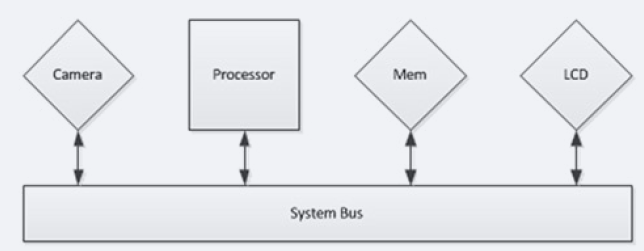
\includegraphics[width=0.45\textwidth]{./pictures/systemArchDiagram.png}
					& 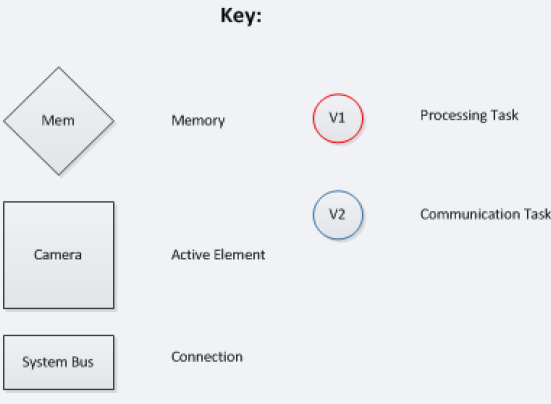
\includegraphics[width=0.45\textwidth]{./pictures/systemArchKey.png}
			\end{tabular}
		\end{table}
		
	\subsection{Bindings}
		\begin{itemize}
		  \item The left part of the binding diagram shows the program flow, with each task as a bubble and arrows that indicate the flow. 
		  \item The right part of the binding diagram shows the system elements, with each element as a bubble. The arrows between the elements are the same data flow connections as in the system architecture diagrams.
		  \item The arrows between the left and the right side of the binding diagram indicate which elements are affected by which tasks.
		\end{itemize}
		
		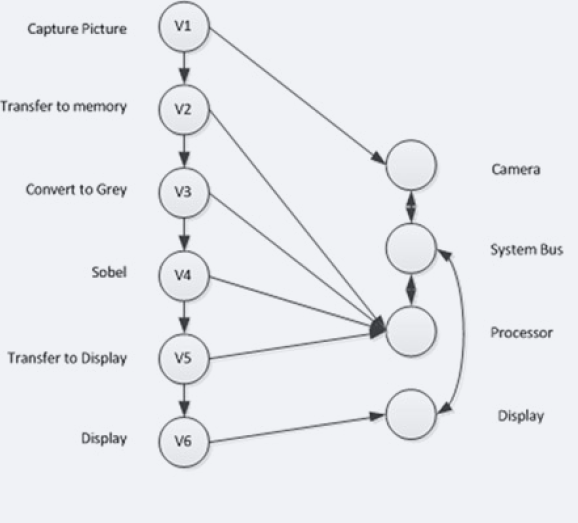
\includegraphics[width=0.45\textwidth]{./pictures/bindings.png}
		
	\subsection{Scheduling}
		\begin{itemize}
		  \item The scheduling diagram indicates how much time is necessary for each of the tasks, how much time is left until the cycle time is is reached and which system architecture element is affected by which task.
		  \item If the same task is affected by multiple elements, that is indicated by showing that this runs at the same time, not after one another. Otherwise it should be split into multiple tasks.
		  \item The tasks in the scheduling diagram are the same tasks as drawn in the left part of the binding diagram.
		\end{itemize}
		
		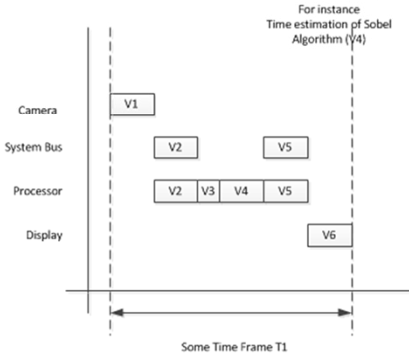
\includegraphics[width=0.45\textwidth]{./pictures/scheduling.png}
		
		\subsubsection{Scheduling Time Measurements}
		\begin{table}[H]\centering
			\begin{tabular}{|p{0.25\linewidth}|p{0.7\linewidth}|}
				\hline
					\textbf{Slack}
						& The time that is left until the maximum cycle time is reached.\\
				\hline
					\textbf{Idle time}
						& The time that the CPU is waiting for other elements to finish their tasks.\\
				\hline
					\textbf{Maximum task scaling factor}
						& The factor, by which the time spent in the CPU's tasks can be multiplied so that the idle time is exactly what the other elements require while the CPU is idle: \newline 
						$T_{IdleNew} = T_{CycleMax} - x \cdot T_{CPU} = T_{OtherElem}$ \newline 
						{\Large $x = \frac{T_{CycleMax} - T_{OtherElem}}{T_{CPU}}$} \\
				\hline
			\end{tabular}
		\end{table}
		
		\subsubsection{List Scheduling}
			The algorithm of list scheduling goes as follows:
			
			\begin{enumerate}
				\item Order tasks with decreasing priority.
				\item Repeat until a valid schedule is obtained:
				\begin{enumerate}
				  \item Select the task with the highest priority.
				  \item Select a resource to accommodate this task.
				  \item If no resource can be found, select next task in the list.
				\end{enumerate}
			\end{enumerate}